\begin{figure}[H]
\begin{subfigure}{.25\textwidth}
  \centering
  \includegraphics[width=.7\linewidth, angle =-90]{img/avg499999stableb.eps}
  \caption{Stable environment.}
\end{subfigure}%
\begin{subfigure}{.25\textwidth}
  \centering
  \includegraphics[width=.7\linewidth, angle =-90]{img/avg499999variationb.eps}
  \caption{Strong Fluctuation.}
\end{subfigure}

\begin{subfigure}{.25\textwidth}
  \centering
  \includegraphics[width=.7\linewidth, angle =-90]{img/avg499999variationLightb.eps}
  \caption{Light Fluctuation.}
\end{subfigure}%
\begin{subfigure}{.25\textwidth}
  \centering
  \includegraphics[width=.7\linewidth, angle =-90]{img/avg499999variationSmallb.eps}
  \caption{Small Fluctuation.}
\end{subfigure}
\caption{Density of Genotype : Each genotype density is processed in four possible different environments.}
\label{fig:density}
\end{figure}


\subsection{Phenotypic Diversity} 
The phenotypic diversity measured in Figure \ref{fig:phenodiv} can also be observed relatively easily by simple observation of the cellular automaton as it can be seen with a few examples in Figures \ref{fig:phenoexpl}. 



\begin{figure}[H]
\begin{subfigure}{.25\textwidth}
  \centering
  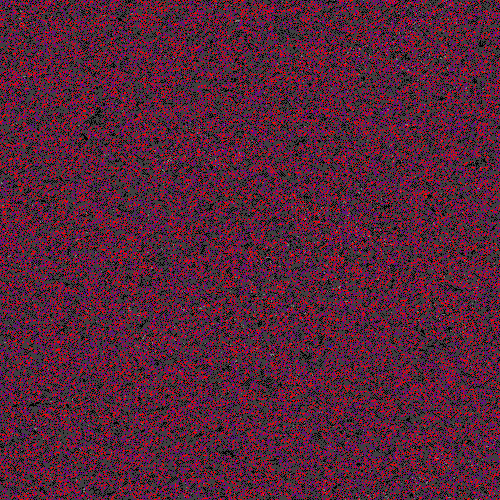
\includegraphics[width=.9\linewidth]{img/stable495000}
  \caption{Stable environment.}
\end{subfigure}%
\begin{subfigure}{.25\textwidth}
  \centering
  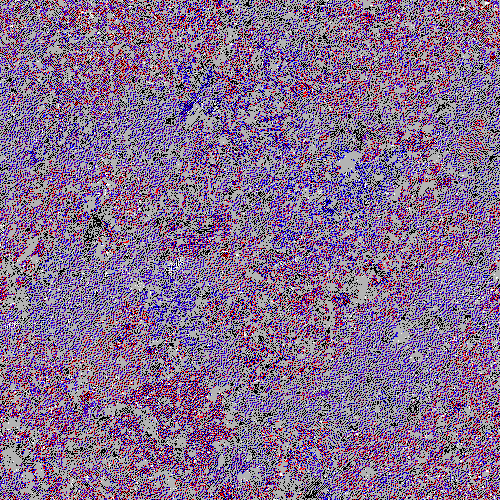
\includegraphics[width=.9\linewidth]{img/var495000}
  \caption{Strong Fluctuation.}
\end{subfigure}

\begin{subfigure}{.25\textwidth}
  \centering
  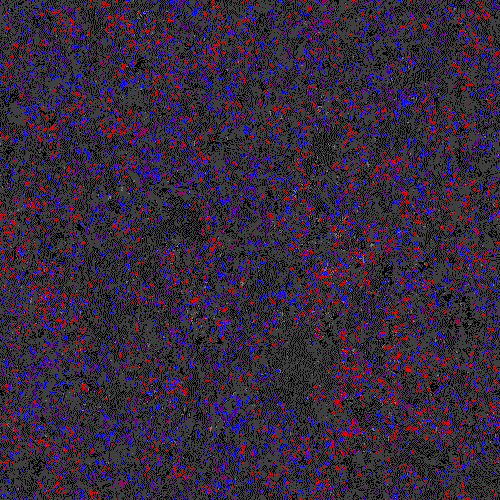
\includegraphics[width=.9\linewidth]{img/light495000}
  \caption{Light Fluctuation.}
\end{subfigure}%
\begin{subfigure}{.25\textwidth}
  \centering
  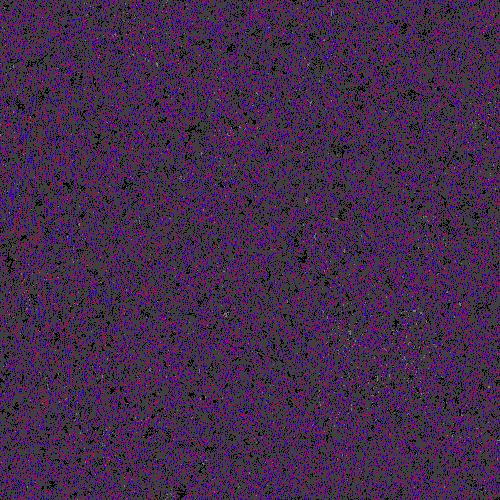
\includegraphics[width=.9\linewidth]{img/small495000}
  \caption{Short-Cycle Fluctuation.}
\end{subfigure}
\caption{Exemple of CA gird state repartition (phenotype) at iteration 495000 for the four different configuration.}
\label{fig:phenoexpl}
\end{figure}


One distinguishes \emph{Strong and Light fluctuations} from \emph{Short-Cycle fluctuations}. These two groups diverge substantially in their characteristic and differ in addition from \emph{Stable Environment}, frequently in between. Individuals from \emph{Short-Cycle fluctuations} seem to produce stable and robust phenotypes in any environment encountered in \emph{Short-Cycle fluctuations}. Their adaptations seem essentially be by genotypic mutations and their plasticity seems low. They are also very dependent on their original ecosystem, sometime very distinctive as depicted in Figure \ref{fig:smalldistinctive}, and consequently very little robust in other types of fluctuations, the effect of genotypic mutations is probably enhanced by the reduced size of genotypes. By contrast individuals evolved with \emph{Strong or Light fluctuations} appear to have a considerable plasticity, their phenotypic diversity is high and it seems likely that phenotypic selection occurs however their genotypic diversity is lower.

\begin{figure}[H]
\begin{subfigure}{.25\textwidth}
  \centering
  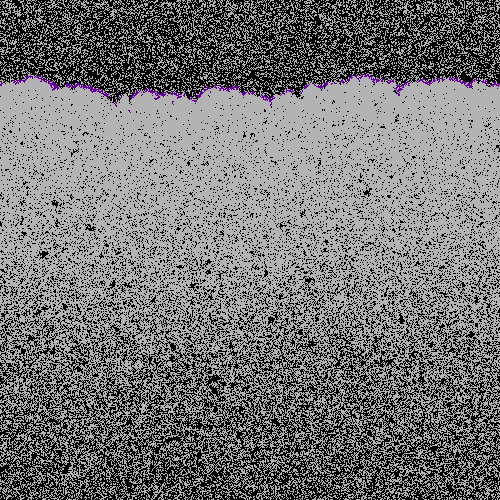
\includegraphics[width=.9\linewidth]{img/sm100000}
  \caption{Iteration 100000.}
\end{subfigure}%
\begin{subfigure}{.25\textwidth}
  \centering
  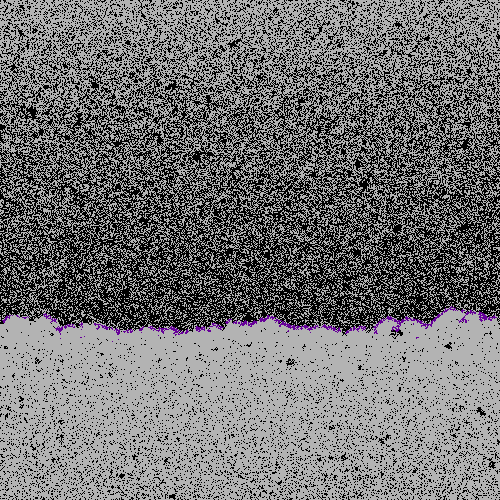
\includegraphics[width=.9\linewidth]{img/sm200000}
  \caption{Iteration 200000.}
\end{subfigure}

\begin{subfigure}{.25\textwidth}
  \centering
  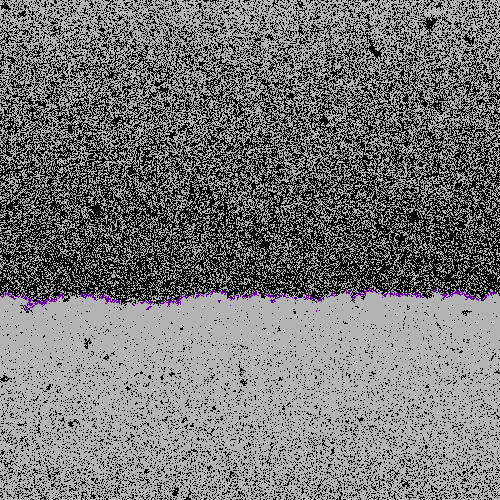
\includegraphics[width=.9\linewidth]{img/sm400000}
  \caption{Iteration 400000.}
\end{subfigure}%
\begin{subfigure}{.25\textwidth}
  \centering
  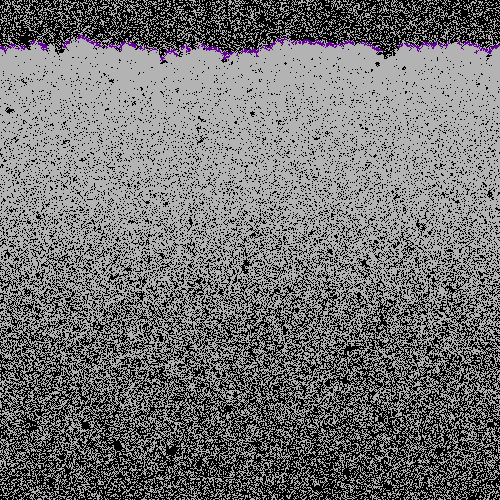
\includegraphics[width=.9\linewidth]{img/sm500000}
  \caption{Iteration 500000.}
\end{subfigure}
\caption{Original \emph{Short-Cycle Fluctuation} simulation having a distinctive waving phenotype, very stable over time, and producing genotypes failing in early iteration of homogeneous test.}
\label{fig:smalldistinctive}
\end{figure}